\documentclass{article}
\usepackage[utf8]{inputenc}
\usepackage{enumitem}
\usepackage{float} % use H for figure placement
\usepackage{pgfplots}
\usetikzlibrary{arrows}
\usepackage{amsmath,amssymb}
\usepackage[margin=1in]{geometry}
\usepackage{hyperref}
\usepackage[amsthm]{ntheorem}
\usepackage{xcolor}
\usepackage{framed}
\definecolor{shadecolor}{rgb}{0.95,0.95,0.95}
\usepackage{physics}

\newtheorem{theorem}{Theorem}[section]
\newtheorem{prop}{Proposition}
\newtheorem{corollary}{Corollary}
\newtheorem{lemma}{Lemma}
\newtheorem{ex}{Example}
\newtheorem*{remark}{Remark}
\theoremstyle{definition}
\newtheorem{definition}{Definition}[section]

\usepackage [autostyle, english = american]{csquotes}
\MakeOuterQuote{"}
\newcommand{\Section}[1]{\hrule\hrule\section{#1}}
\newcommand{\Def}[2]{
\begin{shaded*}
\begin{definition}{\textit{#1}}\\#2\end{definition}
\end{shaded*}
}
\DeclareMathOperator*{\argmin}{arg\,min}
\DeclareMathOperator*{\argmax}{arg\,max}
\def\R{\mathbb{R}}
\def\C{\mathbb{C}}

\title{ENM 521 - MechE Math part 2 - Cheat sheet}
\author{Rebecca Li}
\date{Fall 2019}

\begin{document}
	\maketitle


\raggedright
\footnotesize
\begin{multicols}{3}
	\setlength{\premulticols}{1pt}
	\setlength{\postmulticols}{1pt}
	\setlength{\multicolsep}{1pt}
	\setlength{\columnsep}{2pt}
\section{tricks}
Take the derivative
Bound to zero
Do contours around the branch cut (keyhole)

\section{Common functions}
\begin{itemize}
	\item $e^z = \sum_{n=0}^\infty \frac{z^n}{n!}$
	\item $\sin x = \frac{e^{ix} - e^{-ix}}{2i}$, $\dv{x} asin x = \frac{1}{\sqrt{1-x^2}$
	\item $\cos \frac{e^{ix} + e^{-ix}}{2}$, $\dv{x} acos x = \frac{-1}{\sqrt{1-x^2}$
	\item $\dv{x} atan x = \frac{1}{1+x^2$
	\item $\sinh x = \frac{e^{x} - e^{-x}}{2}$
	\item $\cosh x = \frac{e^{x} + e^{-x}}{2}$
	\item $\sin z = \sin x \cosh y + i \cos x \sinh y$, $\cos z = \cos x \cosh y - i \sin x \sinh y$
	\item $|\sin z|^2 = \sin ^2 x + \sinh ^2 y$, $|\cos z|^2 = \cos ^2 x + \sinh ^2 y$
	\item $\log z$ :  B.P. at 0,$\infty$. $D[\log x] = 1/x$. 
	\item $\lim_{\epsilon \to 0} $$\epsilon \log \epsilon$ = 0
	\item L'hopital's rule 
	\item Funny trig rule 
	\item Geometric series 
\end{itemize}

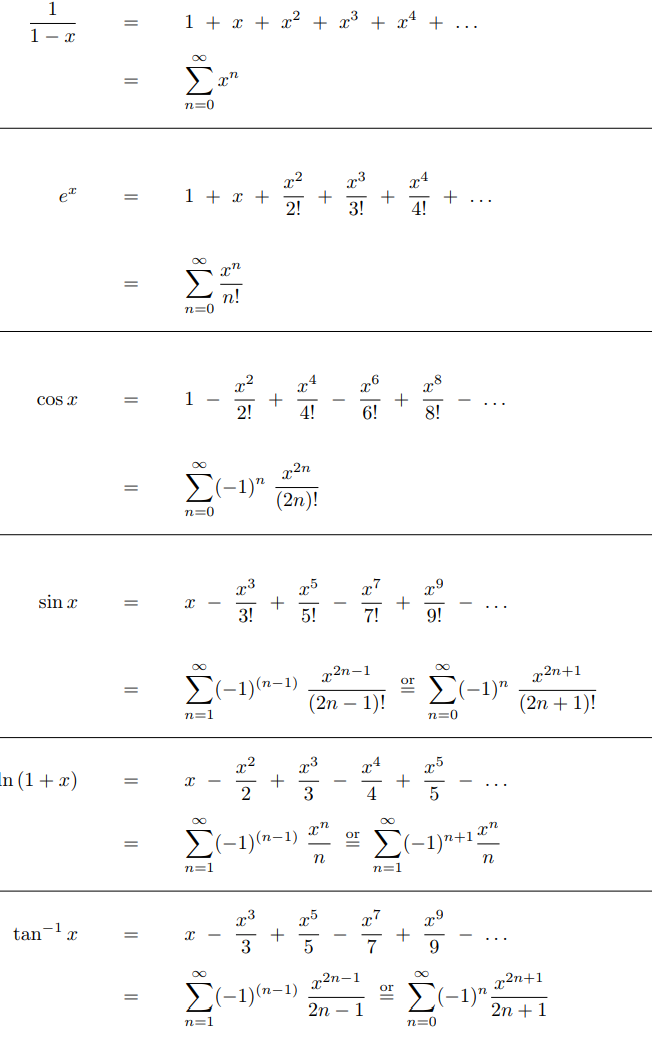
\includegraphics[width=0.7\linewidth]{common_taylor_series}



\section{Sequences}
\textbf{Convergent sequence:}A sequence $\{z_n\}$ is said to have a limit $z_0$ or converge to $z_0$ which we write as 
	
	$$\lim_{n\to\infty} z_n = z_0$$
	
	if for every $\epsilon > 0, \exists\ M \in  \mathbb{Z}$, such that:
	
	$$|z_n - z_0| < \epsilon,\ \forall n > M$$

\textbf{Cauchy Sequence:} a sequence $\{z_m\}$ of complex numbers is a Cauchy sequence if for every $\epsilon>0$, $\exists N \in \mathbb{Z}$ such that $|z_m - z_M| < \epsilon,\ \forall m, M>N$.

\textbf{Cauchy Criterion for Series Convergence} Let $s_m = \sum_{k=1}^{m}a_k$. The series $\sum_{k=1}^{\infty}a_k$ converges if and only if for every $\epsilon>0$, there exists $N \in \mathbb{Z}$ for $m, M>N$:

$$|s_M - s_m| = \left|\sum_{k=m+1}^{M}a_k\right| < \epsilon$$

Alternatively, letting $M = m+p$:

$$|s_{m+p} - s_m| = \left|\sum_{k=m+1}^{m+p}a_k\right| < \epsilon, \forall p = 1,2,3,..$$

This is the most general test for convergence of a series. 
\textbf{Radius of Convergence}:The power series $\sum_{m=0}^\infty a_m z^m$ has a radius of convergence $R = \frac{1}{A}$, where $A =\lim\sup_{m \to \infty } |a_m|^{1/m}$. If $A = \infty$, $R = 0$. Likewise, if $A=0$, $R = \infty$.

\begin{theorem}[Weirstrass M-test]
	Let $M_m$ be a sequence of real numbers. Suppose that $|f_m(z)| < M_m, \forall z \in E, m\in \mathbb{Z}^+$.  If $\sum_{m=1}^\infty M_m$ converges, then $\sum_{m=1}^\infty f_m(z)$ converges uniformly and absolutely on $E$. 
\end{theorem}
 
\textbf{Harmonic function}: Satisfies $\pdv{^2u}{x^2} + \pdv{^2u}{y^2} = 0$
\textbf{Analyticity}: Differentiable everywhere in neighborhood of point.
\textbf{Roots of Unity}: The $k$th root of unity is $\omega$ s.t. $\sum_{n=1}^{k} w^n =0$
\textbf{Entire Function} (TODO)


\section{Branch Points and Branch Cuts}
NOTE: only have to say what it is. 
\begin{itemize}
	\item $z^p$, $p$ non integer has BP at 0, $\infty$.
	\item $\log z$ BP at 0, $\infty$
\end{itemize}
\section{Singularities}
Isolated singularities
\begin{itemize}
	\item \textbf{Pole}: $f$ can be writen as $g/(z-z_0)$
	\item \textbf{Removable}: $z_0$ is analytic in neighborhood and limit exists. Chuanpeng says this is not a singularity.
	\item \textbf{Essential} Neither, yet isolated. Ex. $f(z) = \frac{\sin z}{z}$.
\end{itemize}
Non-isolated singularities 

\section{Taylor/Maclaurin series expansion}
Maclaurin is just taylor about $z=0$.

\section{Laurent Series Expansions}
Two cases:
\begin{enumerate}
	\item $f$ analytic in circle around expansion point. Use Taylor Series Expansion.
	\item $f$ analytic in annulus. Then find Laurent series through something like change of variables to get series.
\end{enumerate}
\textbf{Gauss Mean Value}:
Suppose $f(z)$ is analytic in the closed disk $|z-z_0| \leq r$. Then:
$$f(z_0) = \frac{1}{2 \pi } \int_{0}^{2\pi} f(z_0 + r e^{i\theta} d\theta)$$

\textbf{Cauchy Integral Formula}
If $f$ analytic, $C$ simply connected and closed, $z_0 \in C$, then $f(z_0) = \frac{1}{2\pi i}\int_{C} \frac{f(z)}{z-z_0}dz$. Also $f^{(n)}(z_0) = \frac{n!}{2\pi i } \int_C \frac{f(z)}{(z-z_0)^{n+1}}dz$

\textbf{Cauchy Riemmann Equations} Necessary but NOT sufficient for differentiability at a point. Applied to neighborhood is sufficient for analyticity. Or if $u, v$ have continuous partials in domain $D$. 
Given $f(z) = u(x,y)+iv(x,y)$:
$$\frac{\partial u}{\partial x} = \frac{\partial v}{\partial y},\ \frac{\partial v}{\partial x} = -\frac{\partial u}{\partial y}$$
OR

$$f'(z) = \frac{\partial f}{\partial x} = -i \frac{\partial f}{\partial y}$$
OR 
Let $f=u+iv$ be differentiable with complex partials at $z=re^{i\theta}$. Then:
$$\pdv{u}{r} = \frac{1}{r} \pdv{v}{\theta},\ \pdv{v}{r} = -\frac{1}{r} \pdv{u}{\theta}$$


\textbf{Indented Path lemma}
Let $f$ have a simple pole at $a$ with a residue $\Res[f;a]$. Then given an upper half clockwise semi-circular contour around the pole $C_\epsilon$, the resulting contour is:

\begin{align}
\lim_{\epsilon\to0} \int_{C_\epsilon} f(z) dz = -\Res[f;a]\pi i
\end{align}

\textbf{Jordan's Theorem}: If the only singularities in $g(z)$ are poles, $a>0$, and $g(z) \to 0$ as $R \to \infty$, then 

$$\lim_{R \to \infty} \int_{C_R}e^{iaz}g(z) dz = 0$$

\textbf{Residue theorem}: Suppose that $f(z)$ is analytic inside and on a simple closed contour $C$ except for isolated singularities at $z_1, z_2,..,z_n$ inside $C$. Let the residues at these points be $\alpha_1, \alpha_2,..,\alpha_n$ respectively. Then:
$\int_C f(z) dz = 2 \pi i \sum_{i=1}^n \alpha_i$


Example of sector integration

\textbf{Example log expansion}:Find the Maclaurin expansion of $f(z) = \log(z+1)$ valid for $|z|<1$. We know that $f'(z) = \frac{1}{1+z}$. This is just the same as a geometric series: $f'(z) = \sum_{n=0}^\infty (-1)^n z^n$

Hence:

\begin{align}
f(z) &= \log(1+z) \\ 
& = \int_{0}^z f'(\zeta) d\zeta + f(0) \\ 
& = \sum_{n=0}^\infty \int_{0}^z (-1)^n\zeta^n d\zeta + 0 \\ 
&  = \sum_{n=0}^\infty \frac{(-1)^n\zeta^{n+1}}{n+1}  
\end{align}


\end{document}


